\documentclass[12pt]{article}
\usepackage{natbib}
\usepackage{hyperref}
\usepackage{graphicx}
\usepackage{subcaption}
\usepackage{amssymb,amsmath,amsthm}
\usepackage{xcolor}
\usepackage{xspace}
\usepackage[nameinlink,capitalize]{cleveref}
\usepackage{cleveref}
\usepackage[margin=1in]{geometry}
\usepackage{lineno}\renewcommand\thelinenumber{\color{gray}\arabic{linenumber}}
\usepackage{pdflscape}
\usepackage{xspace}
\usepackage{array}

\newcolumntype{L}[1]{>{\raggedright\let\newline\\\arraybackslash\hspace{0pt}}m{#1}}
\newcolumntype{C}[1]{>{\centering\let\newline\\\arraybackslash\hspace{0pt}}m{#1}}
\newcolumntype{R}[1]{>{\raggedleft\let\newline\\\arraybackslash\hspace{0pt}}m{#1}}

\newcommand{\comment}{\showcomment}
\newcommand{\showcomment}[3]{\textcolor{#1}{\textbf{[#2: }\textsl{#3}\textbf{]}}}
\newcommand{\nocomment}[3]{}

\newcommand{\ali}[1]{\comment{magenta}{Ali}{#1}}
\newcommand{\bmb}[1]{\comment{red}{BMB}{#1}}
\newcommand{\todo}[1]{\comment{red}{TODO}{#1}}

\theoremstyle{definition} % amsthm only
\newtheorem{proposition}{Proposition}
\newtheorem{theorem}{Theorem}
 
\bibliographystyle{apalike}

\title{Centrality: A Curve-Based Statistical Discription of an Ensemble}
\author{Ali Gharouni, Ben Bolker}
\begin{document}
\maketitle
\linenumbers

% %%%%%%%%%%%%%%%%%%%%%%%%%%%%%%%%%%%%%%%
\section{Introduction}

\cite{juul2021fixed} presented a useful curve-based alternative to the fixed-time statistics. 
They cautioned that standard pointwise (fixed-time) averages may not be appropriate to summerize ensembles of epidemic curves. Particularly, miscapturing a key feature such as peak numbers of infections which may result in obscuring the forcast process has been discussed.

\section{Results}

\begin{figure}[h!]
\centering
\begin{subfigure}[t]{.45\textwidth}
\centering
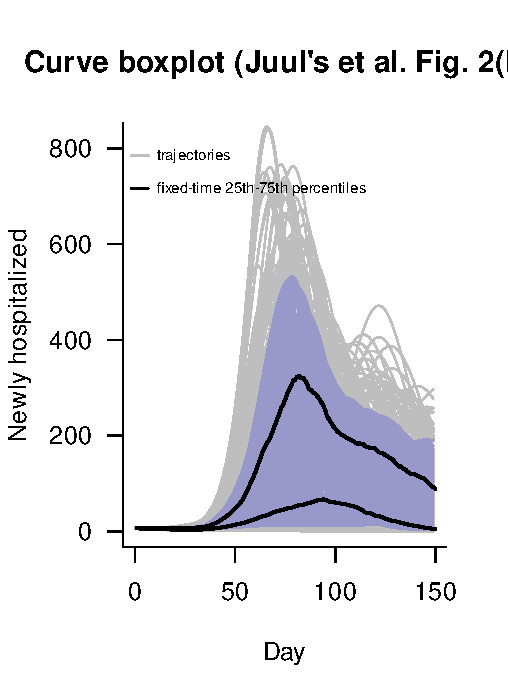
\includegraphics[width=\linewidth]{scripts/pix/fig2b_juul.pdf}
\caption{}\label{p.a}
\end{subfigure}
%
\begin{subfigure}[t]{.45\textwidth}
\centering
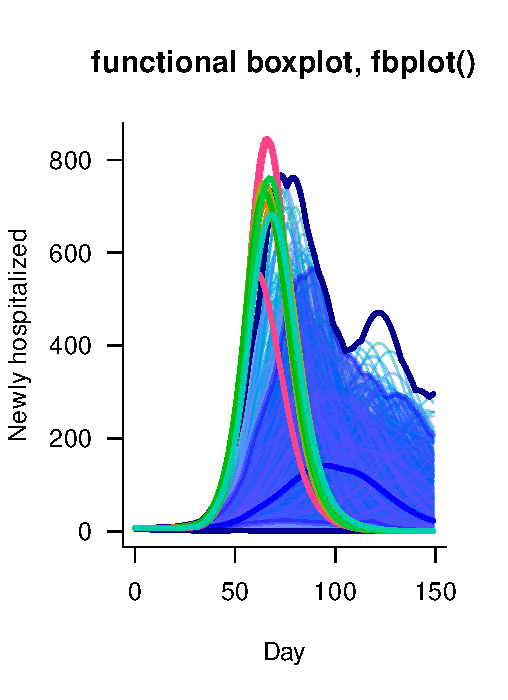
\includegraphics[width=\linewidth]{scripts/pix/fbplot_juul.pdf}
\caption{}\label{p.b}
\end{subfigure}
%
\begin{subfigure}[t]{.45\textwidth}
\centering
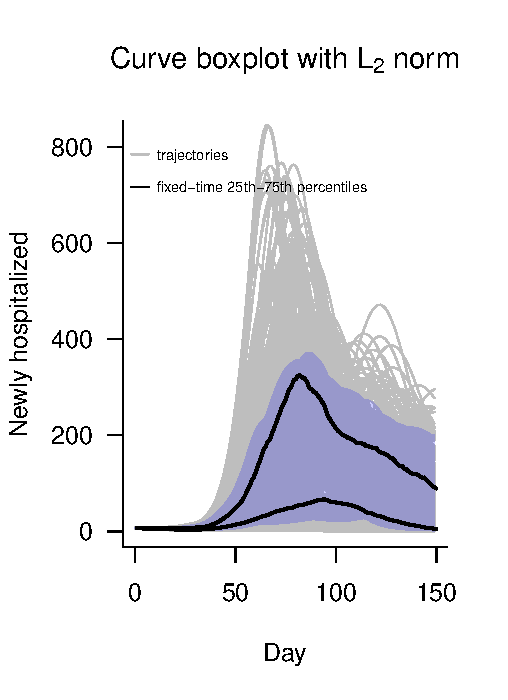
\includegraphics[width=\linewidth]{scripts/pix/L2_juul.pdf}
\caption{}\label{p.c}
\end{subfigure}
%
\begin{subfigure}[t]{.45\textwidth}
\centering
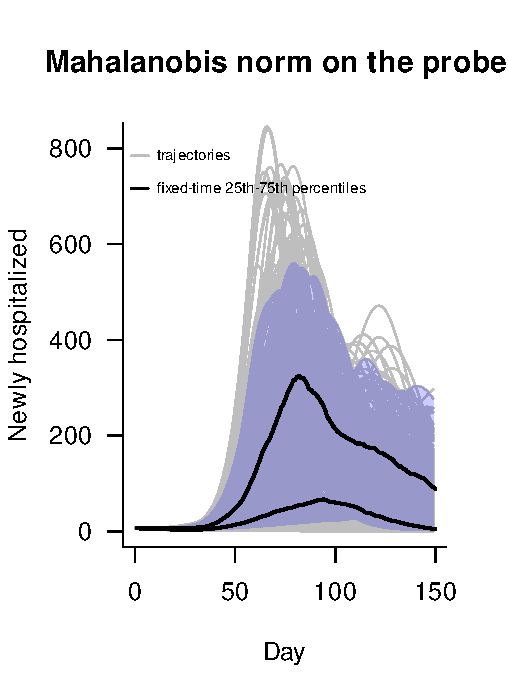
\includegraphics[width=\linewidth]{scripts/pix/mahal_probes_juul.pdf}
\caption{}\label{p.d}
\end{subfigure}
\caption{Other options of curve-based statistics on Juul's et al work}
\label{pan}
\end{figure}


\bibliography{./AliMac}
\end{document}
